\chapter{Experimental Details and Analytical Toolset} \label{ch_exp}
Within this chapter, an overview of the various experimental setups used for the characterization of the samples of this thesis is given. The data evaluated in the course of this thesis resulted from experiments that were performed at the \gls{bessy} and the \gls{mls}, which are third generation synchrotron radiation sources\footnote{In addition to the experiments conducted as part of this thesis, there was \gls{xrr} data taken into account during the analysis. This data was the result of precharacterization experiments done using lab instruments operated by the sample fabricators.}. Depending on the spectral range of the radiation, different beamlines with specialized endstations and different monochromatization methods were used to perform the experiments. The existing experimental setups at the various beamlines and their endstations are reviewed in the following paragraphs. First, an introduction on the basic principles governing the generation of synchrotron radiation and their specific application to metrology tasks is given. Second, the instrumentation at the laboratories of the \gls{ptb} used for the experiments in this thesis is presented.

Additionally, the important details of the multilayer fabrication principle are described as they determine the quality of the sample. The theoretical description from chapter~\ref{ch_theo} already indicated the requirements of optical contrast to achieve high reflectivities of multilayer systems within a certain bandwidth. The details of the sample fabrication and their composition is therefore described in the second part of this chapter.

Finally, a software package was developed to evaluate the data extracted from the measurements and to reconstruct the model parameters describing the layer systems. This software implements all theoretical methods introduced in the previous chapter and allows to quantify structural parameters of the samples based on the experimental data. The last part of this chapter gives a brief description of the individual modules developed in the framework of this thesis.

\section{Synchrotron Radiation}
The radiation emitted by a relativistic charged particle, usually electrons, accelerated on an orbit through an external magnetic field is called synchrotron radiation. This radiation is polarized and emitted tangentially to the orbital movement of the charged particle in forward direction. In the history of synchrotron radiation, sources have evolved from parasitic use of particle accelerators to the extend of building electron storage rings dedicated for the sole purpose of generating this radiation \cite{munro_chapter_1987}. Its most promitent features are the high brilliance, that is the number of photons per second per unit particle beam cross section and per unit solid angle within $0.1\%$ bandwidth at a specific wavelength, and its huge spectral range of emission. Depending on the energy of the relativistic particles forced on an orbit, in modern electron storage rings typically in the order of one to several GeV, the emission covers the range from the terahertz into the hard X-ray regime. The \gls{ptb} operates two laboratories at the dedicated sources \gls{bessy} and \gls{mls} \cite{brandt_metrology_2007}. The two thrid-generation synchrotron radiation sources provide maximum electron energies of $1.7$ GeV (\gls{bessy}) and $0.6$ GeV (\gls{mls}), respectively. Theoretical emission spectra for a single dipole magnet (\emph{bending magnet}) are shown in Fig.~\ref{ch_exp:fig_experimental_synchrotron_spectra} in comparison to black body radiation.
\begin{figure}
 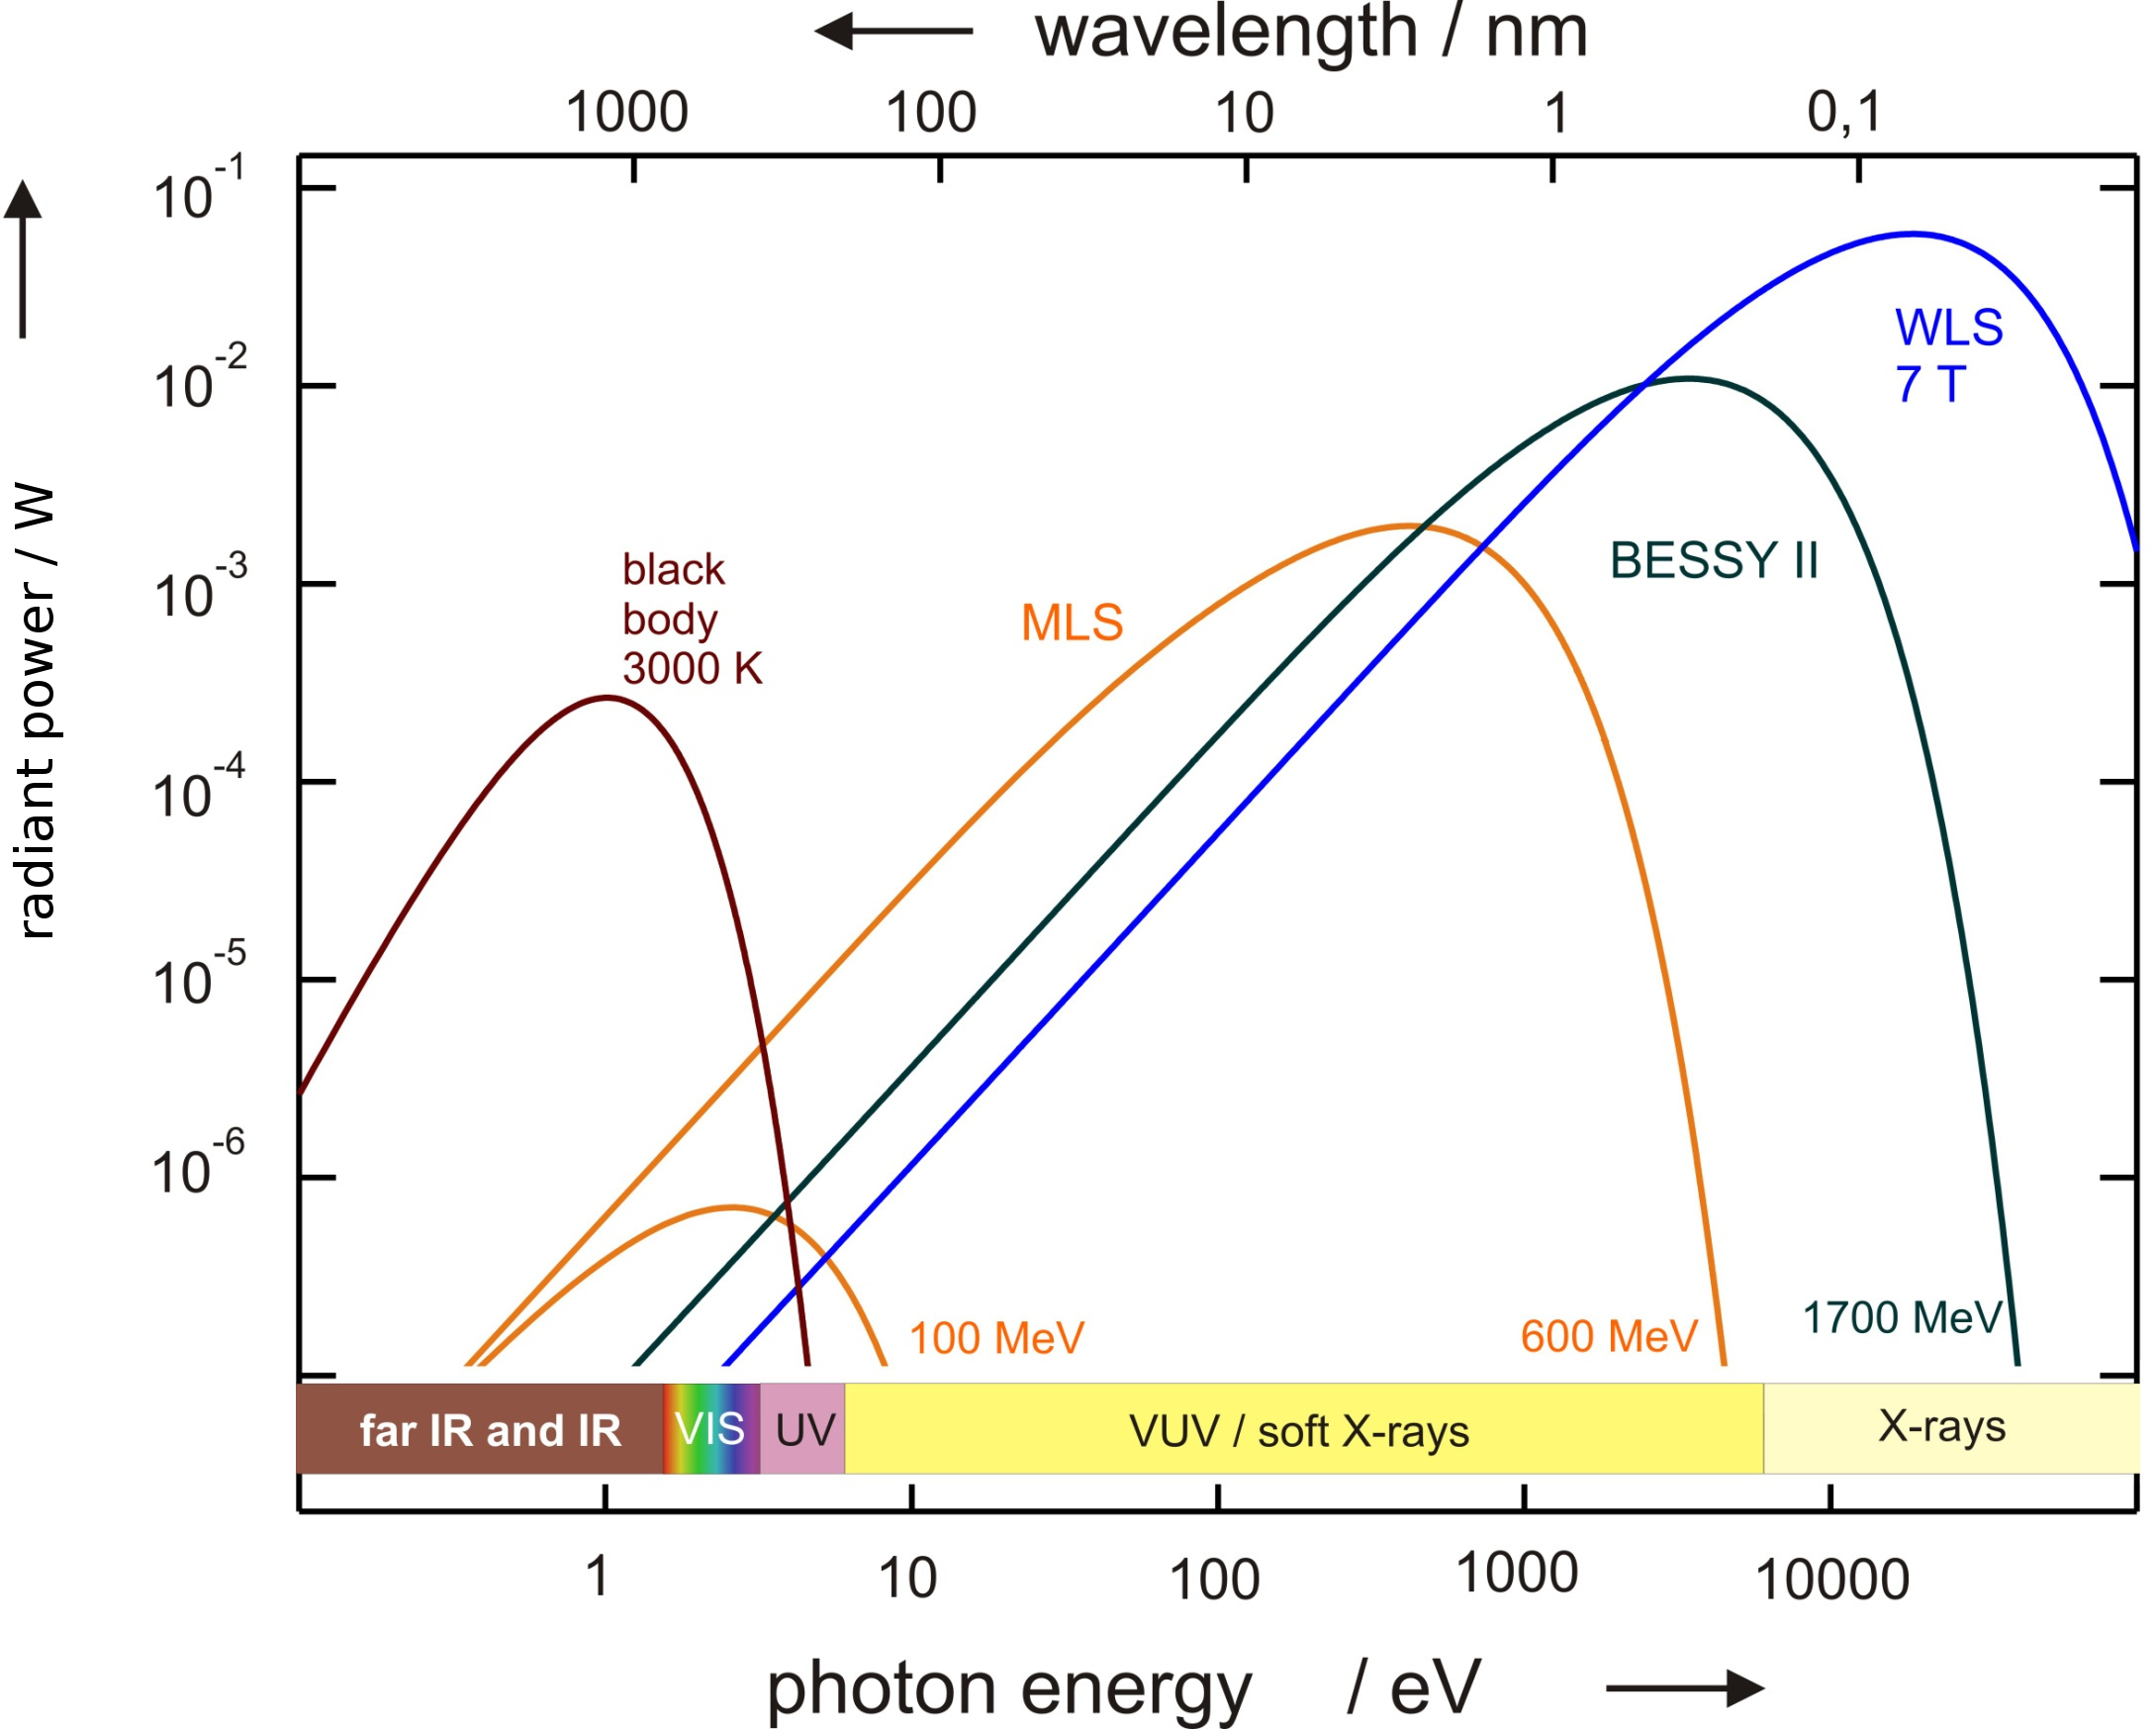
\includegraphics[width=0.7\textwidth]{img/exp-bessy-dipole-spectrum.jpeg}
 \caption[Theoretical synchrotron radiation radiant power spectra]{Theoretical synchrotron radiation radiant power spectra for the \gls{mls} and \gls{bessy} in comparison to black body radiation\footnote{Image taken from \textcite{beckhoff_quarter-century_2009}}. The curves show the radiant power of emission from bending magnets at both electron storage ring facilities for different electron energies. The curve marked WLS shows the radiant power from the $7$ Tesla wavelength shifter insertion device installed at \gls{bessy}.}
 \label{ch_exp:fig_experimental_synchrotron_spectra}
\end{figure}

A very important theoretical aspect of synchrotron radiation, apart from the high brilliance and broad spectrum, is the fact that the emission can be calculated exactly from first principles of classical electrodynamics and special relativity. The theory for synchrotron radiation was developed by Schwinger \cite{schwinger_classical_1949} and we shall review its most imporant aspects here. Given all the fundamental and experimental parameters are known, the total emitted radiant power per relativistic particle can be calculated exactly as
\begin{align}
 P = \frac{1}{4 \pi \gls{epsilon_0}} \frac{2}{3} \frac{\gls{e}^2 \gls{c}}{R^2}\Big( \frac{E}{\gls{m_0} \gls{c}^2}\Big)^4 \text{,} \label{ch_exp:schwinger_equation_total_power}
\end{align}
where \gls{e} is the elementary charge, \gls{c} is the speed of light in vacuum, $E$ is the particles energy, \gls{m_0} is the rest mass of the particle and $R$ is the radius of the circular trajectory imposed by the magnetic field. The radiant power is thus inversely proportional to the fourth power of the particles rest mass, which explains the usage of light electrons in comparison with significanlty heavier protons in synchrotron radiation sources. Apart from the total emitted radiant power, an additional characteristic quantity of synchrotron radiation, visible as a shift to higher photon energies (smaller wavelengths) in Fig.~\ref{ch_exp:fig_experimental_synchrotron_spectra}, is the critical energy or critical wavelength \cite{schwinger_classical_1949}, respectively,
\begin{align}
 E_C = \frac{3 \gls{h} \gls{c}}{4 \pi R} \Big( \frac{E}{\gls{m_0} \gls{c}^2}\Big)^3 \text{.} \label{ch_exp:characteristic_energy}
\end{align}
It marks the point in the spectrum, where the integrated radiant power for all values above and below the critical energy are equal \cite{balerna_introduction_2015}. This formula quantifies the shift towards higher energies due to the increase of the electron energy comparing the \gls{mls} and \gls{bessy} emission spectra. Apart from the spectral distribution, the emitted radiation is linearly polarized with an electric field vector oscillating parallel to the orbital plane. This property, however, is only strictly valid for the emission inside this plane. For radiation above or below, a vertical polarization component (parallel to the surface normal of the orbital plane) exists and the radiation becomes elliptically polarized. The intensity $I(\lambda,\Psi)$ emitted by a single electron on a circular orbit in direction of the azimuthal angle $\Psi$ at the wavelength $\lambda$ is described by
\begin{align}
  I(\lambda,\Psi) &= \frac{27 \gls{e}^2 \gamma^8 }{36 \pi^3 R^3} \Big(\frac{\lambda_c}{\lambda}\Big)^4 \big(1+ (\gamma \Psi)^2\big)\Big( K_{2/3}^2(\zeta) + \frac{(\gamma \Psi)^2}{1 + (\gamma \Psi)^2} K_{1/3}^2(\zeta)\Big) \text{,}
 \label{ch_exp:schwinger_equation_spectral}
\end{align}
where $\gamma = \sfrac{E}{\gls{m_0} \gls{c}^2}$ and $\Psi$ is the angle between the orbital plane and the observation direction outside of that plane \cite{schwinger_classical_1949}. The characteristic wavelength $\lambda_c = \sfrac{h c}{E_c}$ is given by the critical photon energy defined in Eq.~\eqref{ch_exp:characteristic_energy}. The argument of the modified Bessel functions of second kind $K_{x}(\zeta)$ is defined as
\begin{align}
 \zeta = \frac{\lambda}{\lambda_c} \big(1 + (\gamma \Psi)^2\big)^\frac{3}{2} \text{.}
\end{align}


The ability to calculate the exact emission and polarization properties of synchrotron radiation based on Eq.~\eqref{ch_exp:schwinger_equation_spectral} with a given electron current and aceptance angle have another very valuable side effect for the field of metrology. It enables the use of synchrotron radiation as a primary standard for electromagnetic radiation within the available spectral range, which is in fact exploited by the \gls{ptb} \cite{thornagel_electron_2001} to provide absolute radiometry.

The dedicated sychrotron radiation facilities, such as \gls{bessy} and the \gls{mls} provide additional possibilities of generating synchrotron radiation beyond a simple bending magnet through different insertion devices. Fig.~\ref{ch_exp:fig_bessy2} gives a schematic overview of the storage ring \gls{bessy}. At each of the marked dipole magnets, synchrotron radiation is produced according the theory presented above. The radiation is transmitted through outlet systems towards a large number of beamlines, which monochromatize and focus the radiation for experimental applications.
\begin{figure*}[htb]
    \def\svgwidth{0.7\textwidth}
    \import{svg/}{bessy.pdf_tex}
    \caption[Schematic overview of BESSY II.]{Schematic overview of the electron storage ring facility \gls{bessy}\footnote{Original image by \gls{hzb}, Ela Strickert, source: \url{https://www.helmholtz-berlin.de/mediathek/bildarchiv/}}. The synchrotron accelerates the electrons coming from the \gls{linac}, which are then injected in the electron storage ring with their full desired energy. Electromagnetic lenses focus and stabilize the beam, as well as deflecting it onto the circular orbit while emitting synchrotron radiation at each dipole (bending) magnet. Cavities reaccelerate the electrons in the storage ring to compensate the energy loss due to the radiation emission.}
    \label{ch_exp:fig_bessy2}
\end{figure*}
Undulators or wigglers are inserted in the straight sections of the \gls{bessy} storage ring with a large number of periodically arranged magnets with alternating polarization forcing the electrons on a beam path alternating in direction, e.g.~on a sinusoidal path.
\begin{figure*}[htb]
    \def\svgwidth{0.7\textwidth}
    \import{svg/}{bending-wiggler-undulator-fel.pdf_tex}
    \caption[Schematic principle of insertion devices.]{TBD\footnote{Image taken from \url{https://www.helmholtz-berlin.de}}}
    \label{ch_exp:fig_bending-wiggler-undulator-fel}
\end{figure*}
The goal of these insertion devices is to shift the critical energy of the storage ring towards higher energies or increase the radiated power (wigglers). Undulators are a limiting case of a wiggler, where the emitted radiation can interfere constructively dramatically increasing the brilliance within a significantly smaller spectral range compared to bending magnets. The different effect of the undulators and wigglers on the generated spectrum is determined by the magnetic field strength $B_0$ and the distance between two identical periodic arrangements of the magnets of alternating polarization $\lambda_0$. The deflection parameter quantifies this relation through $K \propto B_0 \lambda_0$. Undulators typically have deflection parameters with a small value $K$, while in case of wigglers $K$ is very large \cite{munro_chapter_1987}. Technically, the magnetic field strength can be varied by changing the distance (``gap'') between the magnets vertically. By changing the vertical alignment of the magnetic field direction with respect to the beam path, it is even possible to affect the polarization properties of the emitted radiation to obtain circularly or eliptically polarized radiation.
\begin{figure}[htb]
    \def\svgwidth{0.7\textwidth}
    \import{svg/}{mls.pdf_tex}
    \caption[Schematic overview of the MLS]{Schematic overview of the electron storage ring facility \gls{mls}}
    \label{ch_exp:fig_mls}
\end{figure}


The most advanced light source available today, also known as fourth generation source, is following the concept of a \gls{fel} as first invented by \textcite{madey_stimulated_1971}. In that case radiation is produced by a typically single very long undulator after a linear accelerator instead of a comparatively short straight section of a storage ring. The concept was first demonstrated by \textcite{deacon_first_1977}. \Gls{fel} sources produce highly coherent radiation in the x-ray regime. A possible operation scheme is through the principle of \gls{sase} \cite{derbenev_possibility_1982, bonifacio_collective_1984}. In short, the emitted radiation inside the long undulator has a feedback effect on the electron bunch travelling along the beam path. The result is an exponential amplification of the emitted radiation connected with a (random) wavelength within a certain spectral range defined by the undulator properties until a saturation level is reached \cite{milton_exponential_2001}. The resulting emission spectrum shows several strong spikes of amplified wavelengths with a noisy background.

\section{The Instrumentation for the EUV Spectral Range}
\subsection{The EUV Beamlines at BESSYII and MLS}
The application of radiation generated in bending magnets or in insertion devices in synchrotron radiation sources typically requires monochromatization and focusing trough a series of optical elements depending on the experimental requirements or designated use cases. In the specific case of radiation in the \gls{euv} spectral range, quick absorption during propagation under atmospheric conditions is an additional problem to be considered in the technical setup. It is thus neccessary to maintain a high vacuum from the source point to the experiment and the detector. The two \gls{ptb} beamlines for the \gls{euv} spectral range at the two storage rings \gls{bessy} and \gls{mls} operate on the broad spectrum emitted by bending magnets at each facility. The experiments conducted in the framework of this thesis were performed at both beamlines, as they are optimized for different spectral ranges within the \gls{euv} window as defined in the beginning of chapter~\ref{ch_theo}.  Depending on the required spectral range of the respective experiments, those had to be conducted on the respective instrument. Nevertheless, the two beamlines share many technical and design aspects. Thus, the description here will introduce most of these aspects with respect to the SX700 beamline at \gls{bessy}. The differences of the \gls{euvr} at the \gls{mls} will be given below.

\subsubsection{The Soft X-ray Beamline SX700}
The \gls{sx700} at \gls{bessy} provides a monochromatic beam in the spectral range from $\nm{0.7}$ to $\nm{25}$ wavelength (corresponding to photon energy range from $\ev{50}$ to $\ev{1800}$) \cite{beckhoff_quarter-century_2009}. The total radiation power is shown in Fig.~\ref{ch_exp:fig_flux_sx700}. The beam size at the entrance aperture to the reflectometer (experimental end station) is variable only in vertical direction through the setting of the exit slit. In the standard setting, the beam spot is approximately \mm{1} by \mm{1} \cite{scholze_high-accuracy_2001} and can be reduced vertically (grating dispersion direction) to \mm{0.25}, which is the lower limit of the standard settings.
\begin{figure}[htb]
    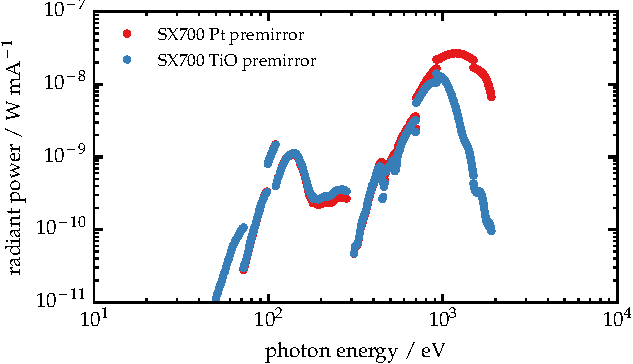
\includegraphics{img/beamline_radiant_power.pdf}
    \caption[Radiant power of the SX700 beamline.]{Radiant power of the SX700 beamline at \gls{bessy} in W per mA storage ring ring current. The two curves differ by the coating on the premirror in the beamline. The Pt coating ensures high radiant power in the high energy range up to \ev{1800}, while the TiO coating absorbs a large amount of high-energy radiation and reduces the radiation power density on the monochromator grating at lower photon energy settings.}
    \label{ch_exp:fig_flux_sx700}
\end{figure}

The monochromatization of the radiation is achieved by a plane grating monochromator with a blazed line grating with 1200 lines per millimeter mounted with its rotational axis parallel to the plane of the storage ring and illuminated perpendicular to the grating lines, yielding the dispersive direction being perpendicular to the storage ring plane. The schematic layout of the beamline is illustrated in Fig.~\ref{ch_exp:fig_sx700_schematic} including the plane grating position of the monochromator, the focussing mirrors and slit positions.
\begin{figure*}[htb]
    \def\svgwidth{\textwidth}
    \import{svg/}{sx700_scheme.pdf_tex}
    \caption[Schematic setup of the SX700 beamline.]{Schematic setup of the \gls{sx700} beamline at \gls{bessy} in top view (upper part) and side view (lower part) \footnote{Original image taken from \textcite{scholze_high-accuracy_2001}}.}
    \label{ch_exp:fig_sx700_schematic}
\end{figure*}
The selection of the desired wavelength is done by the exit slit of the monochromator, which limits vertically and thus allows only a portion of the dispersed radiation to pass through. The achievable relative bandwidth depends on the size of this slit as well as on the selected wavelength. It varies between values of $0.5\times 10^{-3}$ and $2.5\times 10^{-3}$ relative bandwidth. As mentioned above, the monochromator grating disperses the incoming broad band radiation into the vertical direction with respect to the storage ring plane. The blaze of the grating ensures high grating efficiency in the first diffraction order. However, higher diffraction orders are still part of the selected vertical angular range selected by the exit slit leading to a diminished spectral purity. For the purpose of suppression of these higher grating orders, thin metal films in transmission geometry acting as filters are installed close before the exit slit suppressing radiation energetically above the respective absorption edges of the material. In consequence, several different metal thin films have to be used to ensure the spectral purity across the spectral range of the beamline depending on the monochromator setting.

The \gls{sx700} beamline only has one focussing mirror per horizontal and vertical direction, which differs in position in the beamline and produces different focal points for the two directions. The focussing in horizontal direction is done trough the toroidal mirror (cf.~Fig.~\ref{ch_exp:fig_sx700_schematic}), which also serves as a collector mirror for both axis and parallizes the beam in vertical direction. The focal point is located in the entrance aperture (about \m{2} behind the exit slit in propagation direction), which allows to cut off any unwanted stray light at this position. The vertical focussing is done by an additional focussing mirror after the monochromator grating. The vertical focal point is located in the exit slits, which ensures high energy resolution through the selection process explained above. Due to the large distance of the two focussing elements to the experimental station and the low acceptance of the torodial mirror, a low divergence of the beam of about $1.6$ mrad $\times$ $0.4$ mrad is achieved.

\subsubsection{The Extreme Ultraviolet Beamline EUVR}
The general layout and operation principle of the \gls{euvr} beamline is identical to that of the \gls{sx700} beamline described in the previous paragraph with some differences in the focussing and radiant power, which are described in the following. Due to the lower electron energy in the \gls{mls} storage ring, the spectrum of the bending magnets for both beamlines differs with the critical energy shifted to smaller values (cf.~Fig.~\ref{ch_exp:fig_experimental_synchrotron_spectra}). Consequently, the wavelength range covered by the \gls{euvr} beamline is between \nm{5} to \nm{50} (corresponding to photon energies from approximately \ev{25} to \ev{248}), to make use of the higher radiant power available in that range compared to the \gls{bessy} spectrum. The toroidal mirror (collector mirror) of the \gls{euvr} beamline does have a larger aperture and is positioned significantly closer to the source point. Through this modification, an increase of the total acceptance angle by two orders of magnitude is achieved. This, however, increases the divergence of the beam to approximately $4$ mrad in both directions. In contrast to the \gls{sx700} beamline, the foci for horizontal and vertical direction are both at the position of the exit slit with an additional refocusing mirror behind that slit to counteract the strong divergence. Together with the shifted bending magnet spectrum of the \gls{mls}, this different setup allows higher photon flux. In addition, the refocusing allows the spot size of the \gls{euvr} beamline to be adjusted (by closing the cooled apertures shown in Fig.~\ref{ch_exp:fig_sx700_schematic}) at acceptable reduction of the overall photon flux. Furthermore, through an off-center positioning of the cooled aperture opening outside of the orbital plane of the ring, different polarization degrees may be chosen. The key properties of both beamlines and their differences are given in Table~\ref{ch_exp:tbl_beamline_properties}. The optics of both beamlines in comparison are shown in Fig.~\ref{ch_exp:beamline_optics}.
\begin{table*}
\centering
\begin{tabular}{lrr}
\toprule
Parameter 			& \gls{sx700} 		& \gls{euvr}\\ \midrule
Wavelength range 		& $\nm{0.7}$ to $\nm{24.8}$ 	& $\nm{5}$ to $\nm{50}$\\
Spot size (standard settings)			& $\mm{1} \times \mm{1}$ 		& $\mm{0.1} \times \mm{0.1}$ to\\ 
&&$\mm{2} \times \mm{2}$\\
Beam divergence			& $\mrad{1.6}\times \mrad{0.4}$ 	& $\mrad{4}\times \mrad{4}$\\
Linear polarization (horizontal)	& $\SI{98}{\percent}$ 		& $\SI{40}{\percent}$ to $\SI{98}{\percent}$\\
 \bottomrule
\end{tabular}
\caption{Beamline parameters of the two EUV beamlines \gls{euvr} and \gls{sx700} in comparison.}
\label{ch_exp:tbl_beamline_properties}
\end{table*}
\begin{figure*}[htb]
    \def\svgwidth{\textwidth}
    \import{svg/}{beamline_optics.pdf_tex}
    \caption[Schematic optics of the SX700 and EUVR beamlines.]{Schematic optics of the SX700 and EUVR beamlines in direct comparison.}
    \label{ch_exp:beamline_optics}
\end{figure*}

\subsection{The Experimental Endstations at the EUVR and SX700 Beamlines}
All experimenents in the \gls{euv} spectral range within the framework of this thesis were conducted at the beamlines \acrshort{euvr} and \acrshort{sx700}. Each of the beamlines is equipped with an experimental end station containing the detectors, mounts for \gls{ccd} cameras and a goniometer to adjust the angle of the sample holder with respect to the beam. Due to the high absorption of the \gls{euv} radiation in air, both chambers need to be kept under high vacuum conditions, typically below the limit of \mbar{3E-6}.

The end stations differ in the size and weight of samples, which can be mounted on the sample holder. The large reflectometer at the \gls{euvr} beamline was designed with heavy and large samples in mind, whereas the ellipso-scatterometer at the \gls{sx700} beamline covers a larger anglular range for both the detector and the sample holder, due to additional axis allowing measurements anywhere in between and including perpendicular to the orbital plane (\emph{s-polarization} direction) and parallel to the orbital plane (\emph{p-polarization} direction). In the following the two different setups with their primary features are summarized. 

\subsubsection{The large reflectometer at the \gls{euvr} beamline}
The large reflectometer serving as the end station at the \gls{euvr} beamline was designed for reflectometry and scatterometry measurements for samples with a weight of up to \SI{50}{\kg} and a maximum diameter of \mm{550} in mind\cite{tummler_characterization_2003}. The available axis of movement and rotation are shown in Fig.~\ref{ch_exp:fig_bigref}.
\begin{figure*}[htb]
    \def\svgwidth{\textwidth}
    \import{svg/}{bigref.pdf_tex}
    \caption[The BigRef.]{The \gls{euv} reflectometer end station of the \gls{euvr} beamline at the \gls{mls}. A photograph of the internal mechanics and the vacuum chamber is shown in (a). The schematic layout of the goniometer axes and the detector arm are shown in (b).}
    \label{ch_exp:fig_bigref}
\end{figure*}
The sample holder plate allows for linear movement in all three orthogonal directions as well as angular rotations in three axis. The rotation around the $\Theta$-axis covers the range from $\SI{-30}{\degree}$ to $\SI{95}{\degree}$ relative to the incoming beam. Thus, enabling reflectometry and scatterometry from normal incidence to grazing incidence angles together with the detector arm rotation around the $2\Theta$-axis from $\SI{-5}{\degree}$ to $\SI{190}{\degree}$. The rotation of the sample holder around the $\phi$-axis (cf.~Fig.~\ref{ch_exp:fig_bigref}) with an angular range from $\SI{0}{\degree}$ to $\SI{360}{\degree}$, allows to measure a sample mounted in the center of the sample holder with radiation impinging from all directions. The distance of the detector to the sample is variable through the \emph{Det-R} axis from a minimum value of $\mm{150}$ to $\mm{550}$.

The detector mount is equipped with up to $4$ diodes, which can be rotated to face either the sample or the incoming beam. The diodes used within the framework of this thesis are $\mm{4.5} \times \mm{4.5}$ and, optionally $\mm{10} \times \mm{10}$, GaAsP photodiodes. The detector holder can be moved along the $\Theta$ and $2\Theta$ rotational axes, labeled as \emph{Det-X} direction in Fig.~\ref{ch_exp:fig_bigref}, which allows to take measurements in the \emph{out-of-plane}\footnote{The out-of-plane scattering direction refers to radiation scattered outside of the scattering plane spanned by the surface normal of the sample and the impinging beam direction.} direction in s-polarization.

\subsubsection{The Ellipso-scatterometer at the \gls{sx700} beamline}
The ellipso-scatterometer is a reflectometer similar to the large reflectometer providing the end station for the \gls{sx700} beamline. Its capabilities differ from the large reflectometer by a wider reachable angular range for both the detector movement as well as the sample movement. The angular and linear movements and axes are shown in Fig.~\ref{ch_exp:fig_elli} together with a photograph of the goniometer and detector arm.
\begin{figure*}[htb]
    \def\svgwidth{\textwidth}
    \import{svg/}{elli.pdf_tex}
    \caption[The EUV ellipso-scatterometer.]{The EUV ellipso-scatterometer end station at the \gls{sx700} beamline at \gls{bessy}. The internal mechanics of the goniometer and the detector arm are shown in (a). The schematic layout of the axes an the movable detector arm are given in (b).}
    \label{ch_exp:fig_elli}
\end{figure*}
In contrast to the large end station at the \gls{euvr} beamline, it can hold samples with a a maximum of $\SI{5}{\kg}$ in weight. However, the rotational movement of both the detector and the sample holder allow for a larger angular range. In particular, the detector holder may be moved on large parts of the upper hemisphere above the sample holder. In consequence, measurements in s-polarization and well as p-polarization can be conducted on the same sample. With the capability to mount a polarization analyzer at the detector holder, polarization resolved measurements are thus possible \cite{soltwisch_polarization_2015}.

\section{Grazing-incidence X-ray Fluorescence at the FCM Beamline} \label{ch_exp:sec_xrf_at_fcm}
The \gls{gixrf} measurements of the Cr/Sc sample systems were performed at the \gls{fcm} bending magnet beamline \cite{krumrey_design_1998} in the \gls{bessy} laboratory. The necessary photon energies to excite the K-edge x-ray fluorescence of chromium and scandium, are well above the spectral range of the \gls{euvr} and \gls{sx700} beamlines in the order of several \si{\kilo\electronvolt}. The general setup and design of the \gls{fcm} beamline is very similar to that of the \gls{sx700} beamline, with the exception of the four crystal monochromator, which replaces the plane grating monochromator in the x-ray spectral range. It offers tunable photon energies from \kev{1.75} to \kev{10.0}. A high energy resolution of $E/\Delta E = 10^4$ is attained by the combination of four exchangeable crystal Bragg reflections. The monochromator can be equipped with two monochromator crystal types. For the high energy range above approximately \kev{3.5} to \kev{10.0} silicon is used. In the lower energy range between \kev{1.75} and \kev{3.5} higher radiant power is available through the usage of a InSb crystal and more specifically, the silicon K-edge at \kev{1.84} becomes accessible. A schematic overview of the \gls{fcm} beamline can be found in Fig.~\ref{ch_exp:fig_fcm_scheme}.
\begin{figure}[htb]
        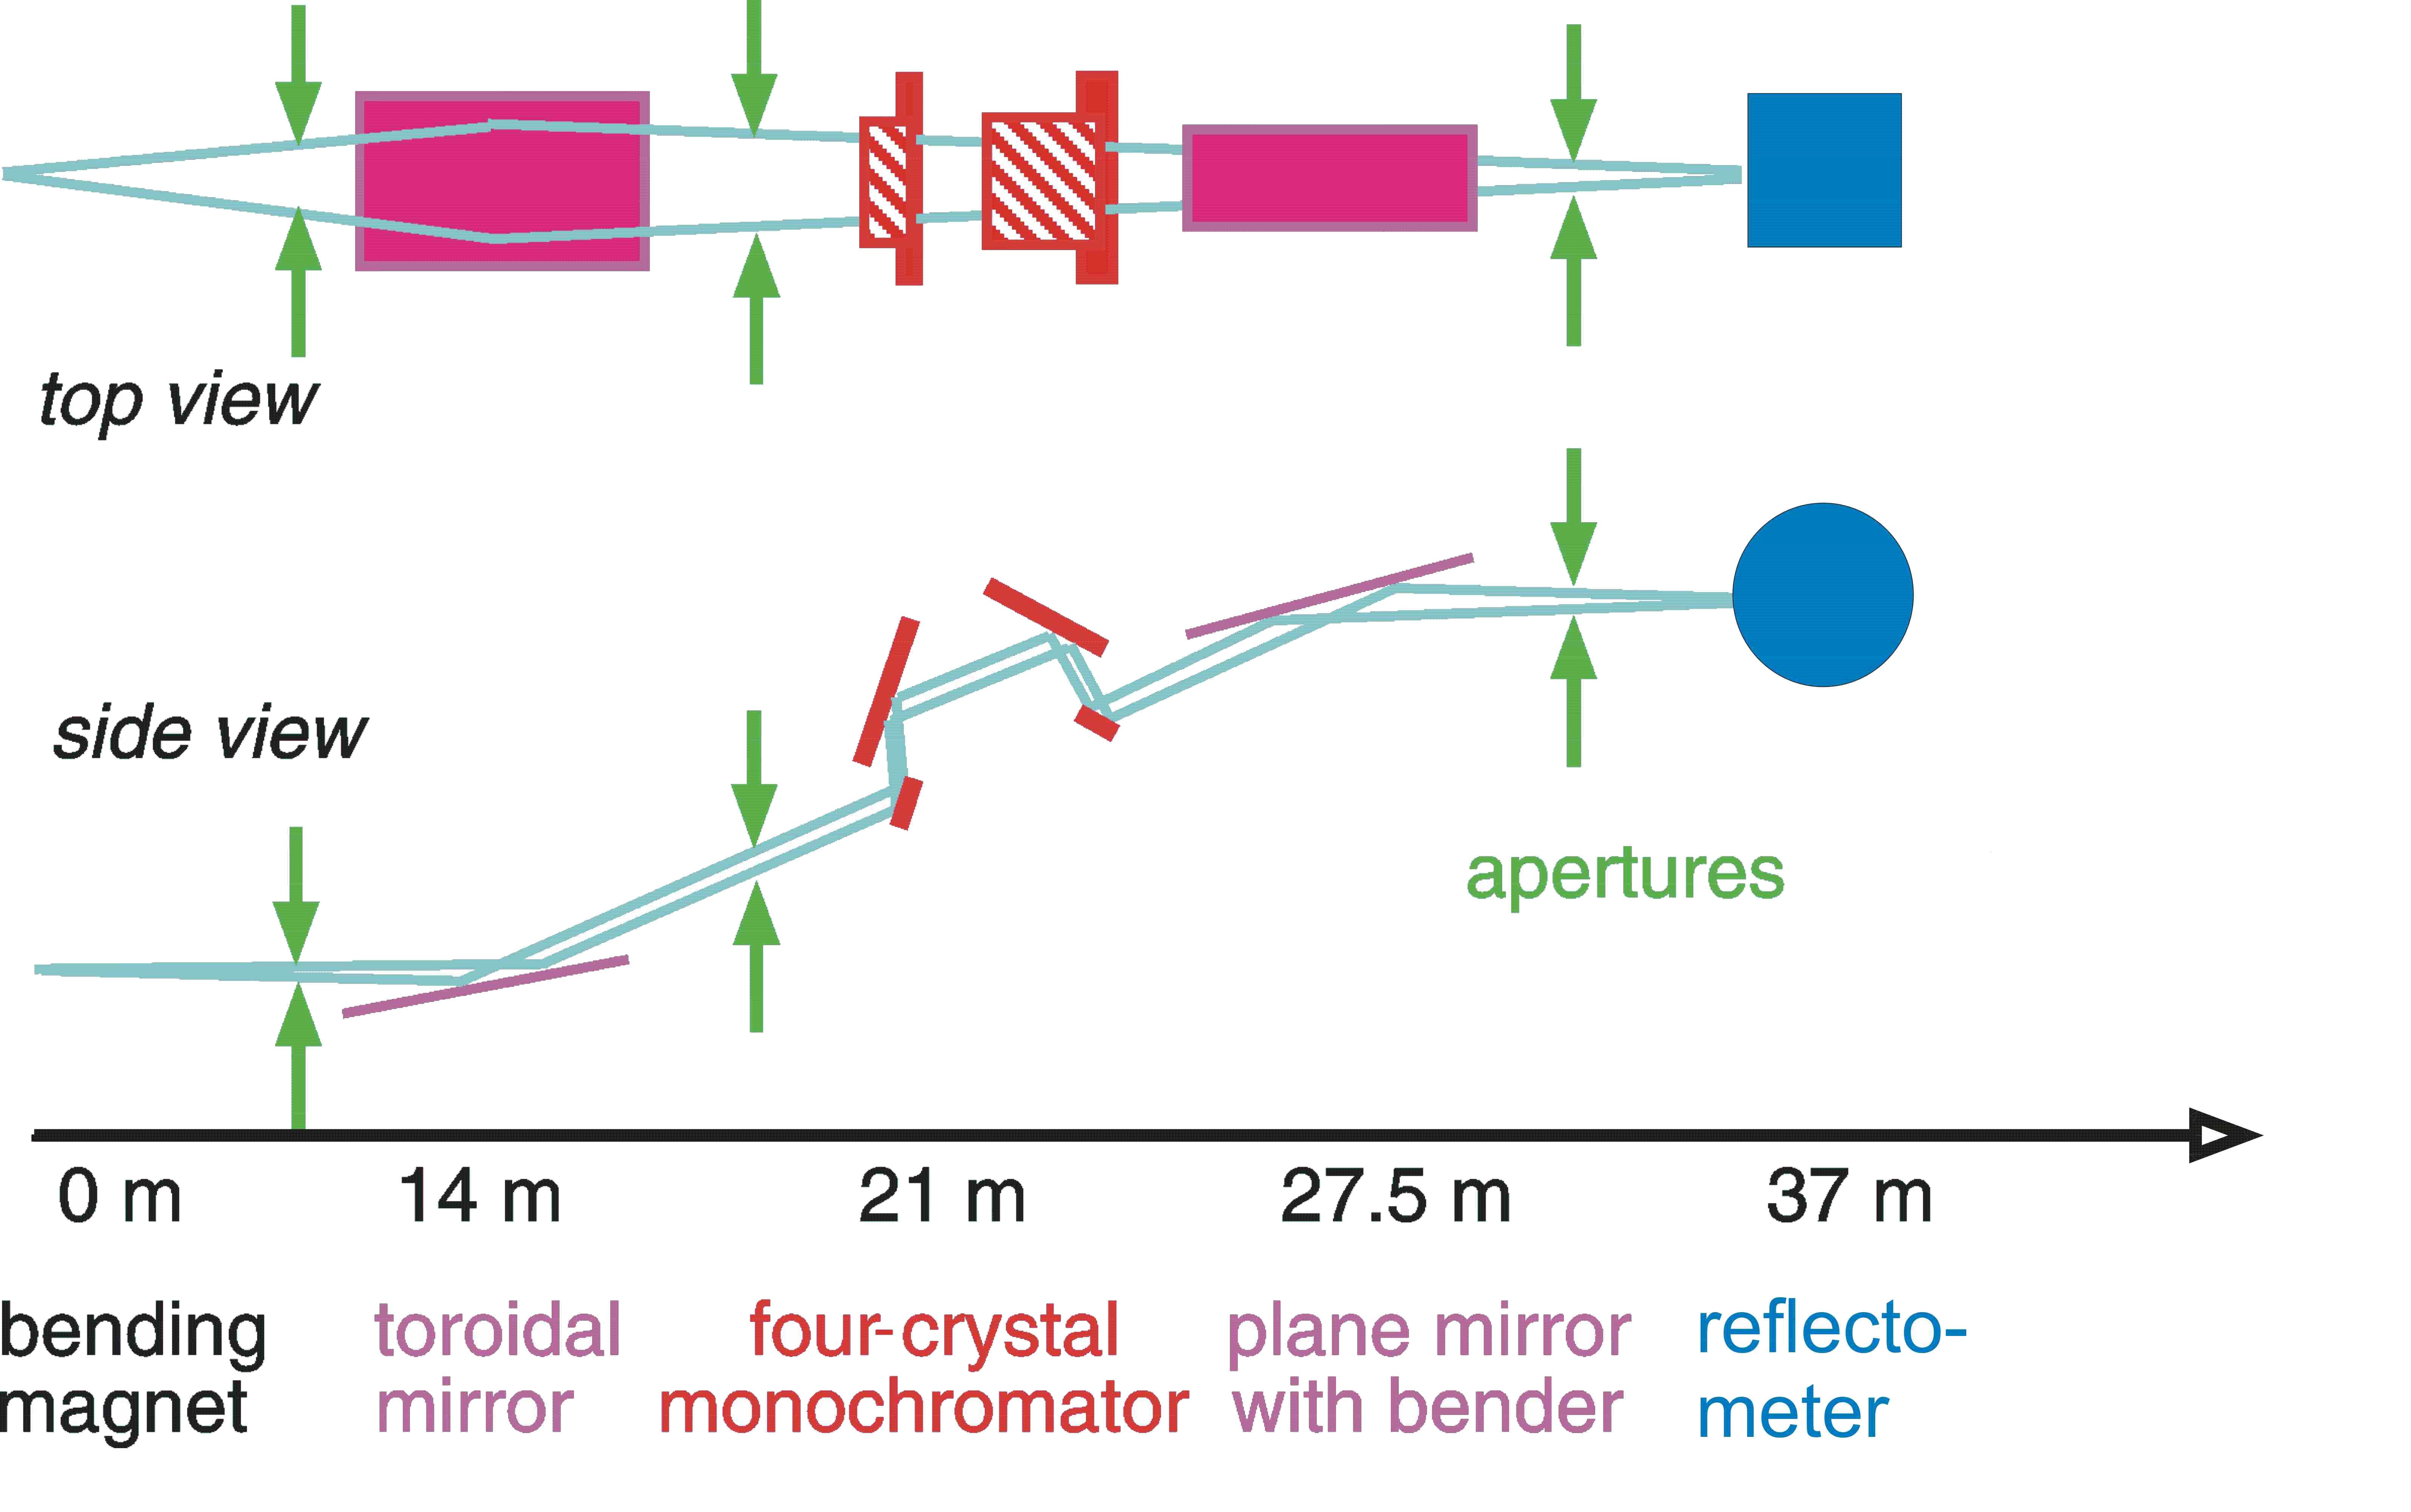
\includegraphics[width=0.7\textwidth]{img/FCMScheme.png}
        \caption[FCM beamline scheme.]{%
            Schematic layout\footnote{Original image taken from \textcite{krumrey_design_1998}.} and optical path of the \gls{fcm} beamline at \gls{bessy}. The setup is comparable to the \gls{sx700} beamline, but uses a four-crystal monochromator setup instead.}
        \label{ch_exp:fig_fcm_scheme}
\end{figure}

The end station used for the \gls{gixrf} experiments is a specialized chamber for \gls{gixrf}, \gls{txrf} and \gls{xrr} \cite{lubeck_novel_2013} depicted in Fig.~\ref{ch_exp:fig_gixrf_chamber}. It is equipped with a detector arm and a sample goniometer allowing to measure grazing incidence angles of \SI{0}{\degree} to \SI{60}{\degree}. The detector arm holds a diode allowing \gls{xrr} measurements. Perpendicular to the beam direction, an energy dispersive \gls{ssd} is mounted close to the sample surface. It allows to detect fluorescence radiation emitted from the sample energetically resolved. The samples can be rotated with respect to the storage ring plane in order to allow a variable polarization impinging on the surface, very similar to the axis movements possible with the ellipso-scatterometer end station at the \gls{sx700} beamline.



\begin{figure*}[htb]
    \def\svgwidth{\textwidth}
    \import{svg/}{gixrf_chamber.pdf_tex}
    \caption[The GIXRF chamber.]{The schematic layout of the dedicated \gls{gixrf} chamber\footnote{Images taken from \textcite{lubeck_novel_2013}.}. This end station can be mounted to the \gls{fcm} or \gls{pgm} beamlines to conduct grazing-incidence \gls{xrf} experiments. In (a), the schematic exterior layout and, in (b), the interior layouts are shown.}
    \label{ch_exp:fig_gixrf_chamber}
\end{figure*}

\section{Sample systems}
The samples studied in the framework of this thesis are designed to work as near-normal incidence mirrors for the \gls{euv} spectral range. The underlying principle of an artificial one dimensional Bragg crystal requires the deposition of thin layered systems with high periodicity and stability. The experiments presented here were conducted on two sets of sample types as prototypes of mirrors for two different spectral ranges. In the theoretical description of the principle of multilayer mirrors in Sec.~\ref{ch_theo:sec_multilayer} of Ch.~\ref{ch_theo} is was outlined, that optical contrast, i.e.~a large as possible difference in the real part of the refractive index $n$, is required to achieve high reflectivities while maintaining a low absorption. The latter is of special importance, as stacking of several layers is only beneficial if the radiation can reach deep into the layer stack. Nevertheless, a compromise between low absorption and optical contrast has to be found specific for the application and the desired spectral range. While high peak reflectivities in a relatively small spectrum require many layers to contribute, broadband mirrors with smaller peak reflectance may work better with a material with higher absorption and higher optical contrast with fewer layers contributing to the reflectivity.


\subsection{Choice of the Chemical Species and Multilayer Design}
\label{ch_exp:sec_multilayer_design}
This thesis investigates systems designed to reflect radiation in two spectral ranges, the \emph{water window} with wavelengths from \nm{2.2} to \nm{4.4} and the range from \nm{12.4} to \nm{14.0} with a wide range of applications, e.g.~for the next-generation lithography. The choice of the chemical species for the multilayer systems, apart from trivial properties such as non-toxicity and solidity, is largely influenced by the electronic structure of the respective materials, since large changes in the refractive index, i.e.~large optical contrast with respect to a second material, can be expected close to resonances in the electronic structure. The demand for low absorption also requires species, where the absorption edges are energetically higher or far lower than the desired spectral range of operation. For a well defined interface it is also necessary that the two materials are mostly inert and do not react with one another or alternatively, if reactive materials are the only reasonable choice, that mechanisms for avoiding strong intermixing exist.

\paragraph{Cr/Sc multilayer system}
In case of the water window spectral range, we investigated samples designed for a peak reflectance at a wavelength closely above \nm{3.14}, where the L3 edge of scandium (Sc) is found. Fig.~\ref{ch_exp:fig_crsc_contrast} shows the refractive index of Sc and the second material chromium (Cr) in the water window spectral range. 
\begin{figure}[htb]
        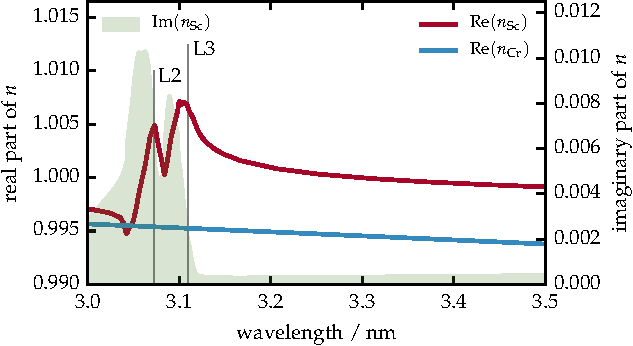
\includegraphics{img/Cr_Sc_contrast}
        \caption[Refractive indices of Cr and Sc in the water window.]{%
            Refractive indices of Cr and Sc with the water window spectral range. The marked absorption edges are the L2 and L3 edge of Sc. The imaginary part of the refractive index accounts for the absorption and is shown for Sc. At wavelengths only slightly larger than that of the L3 edge is the highest contrast for the two materials providing the highest potential reflectivity in a periodic multilayer arrangement.}
        \label{ch_exp:fig_crsc_contrast}
\end{figure}
The periodic multilayers of the systems investigated here, were therefore binary alternating layers of Cr and Sc. The required nominal period thickness $D$, i.e.~the thickness of each periodically repeated layer stack, for the design goal of a peak reflectivity at $\lambda=\nm{3.14}$ is $D=\nm{1.573}$ with a layer thickness ratio of $\Gamma=0.5$ of both materials. To protect the Sc layers from oxidation, an additional Cr capping layer of approximately $d_\text{cap} = \nm{3}$ was added as the surface layer. The multilayer is composed of alternating layers of Cr and Sc with periodic replication of the bilayer stack by $N=400$ times. The substrate is a Si wafer piece. The sample dimensions measure 
approximately $(20 \times 20)$ mm$^2$. More details can be found elsewhere \cite{prasciolu_thermal_2014}. The multilayer mirror was designed to reflect radiation in the water window, at wavelengths just above the Sc L edge, close to a $3.1$ nm at an angle of incidence (AOI) of $\alpha_i = \SI{1.5}{\degree}$.

%The Cr/Sc multilayer samples were prepared at the DESY X-ray multilayer 
%laboratory by DC magnetron sputtering. The deposition was performed at $0.133$ 
%Pa ultrahigh purity Ar ($99.999\%$) and a power of $200$ W for both Sc and Cr 
sputtering targets. 


\paragraph{Mo/Si multilayer systems}
The second set of systems under investigation in this thesis is composed out of $50$ to $65$ bilayers Molymdenum (Mo) and Silicon (Si). Si shows a very low absorption in the range from \nm{12.4} to \nm{14.0}, with the Si L2 edge forming the lower wavelength limit for the usage as a mirror system in this combination. The Mo layers absorb stronger but provide the optical contrast required for high peak reflectance, as outlined at the beginning of this section. The respective refractive indices are given in Fig.~\ref{ch_exp:fig_mosi_contrast}.
\begin{figure}[htb]
        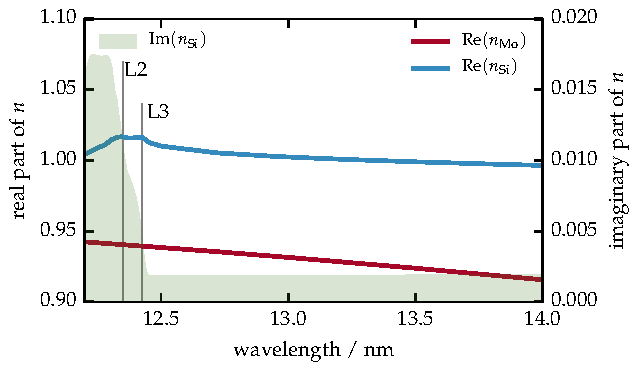
\includegraphics{img/Mo_Si_contrast}
        \caption[Refractive indices of Mo and Si in the wavelength range from \nm{12.4} to \nm{14.0}.]{%
            Refractive indices of Mo and Si in the wavelength range from \nm{12.4} to \nm{14.0}. The L3 absorption edge of Si marks the lower wavelength limit for the applicability of this material combination in multilayer mirror systems.}
        \label{ch_exp:fig_mosi_contrast}
\end{figure}

Finally, specifically Mo and Si are a choice of materials, which indeed do react and form MoSi$_x$ compounds at the interfaces. This reduces the optical contrast and has to be avoided. For that purpuse the sample systems can contain additional materials, which serve as barrier layers preventing this effect. The two species used for our samples are Boroncarbite (B$_4$C) and Carbon (C). Those two materials do not have any absorption edges in the given relevant spectral range and additionally show low contrast to the spacer material Si. The details of the respective sample layouts are discussed in the corresponding sections of the following chapters.

\subsection{Multilayer Deposition by Magnetron Sputtering} \label{ch_exp:sec_magnetron_sputtering}
The multilayer samples investigated here were fabricated by the DC magnetron sputtering technique \cite{stearns_fabrication_1991} by two different multilayer and optics groups. The Mo/Si multilayer samples were fabricated by Stefan Braun at the Fraunhofer IWS, Dresden, Germany and the Cr/Sc samples are by Sa\v{s}a Bajt from the Optics Group at CFEL, DESY, Hamburg in Germany.

Magnetron sputtering is a physical vapor deposition technique. A vacuum chamber is equipped with a substrate to be coated, in our case silicon, and one or more sputter targets. Depending on the intended design of the multilayer to be deposited, those targets are the respective materials, which later form the individual layers. In the DC magnetron sputtering system, a strong electric field is applied between the substrate and the sputter targets. The vacuum chamber containing those parts is then filled with a sputter gas, typically ultrapure Ar gas (\SI{99.999}{\percent}), with partial pressures in the range from \mbar{E-3} to \mbar{E-2} \cite{stearns_fabrication_1991}. The strong electric field ionizes the sputter gas causing the ions to be accelerated towards the sputter targets (cathode) and form a charged plasma. Upon impact in the target, atoms and electrons of the condensed matter phase of the respective material are released and travel towards the substrate. The released atoms condense there, forming bonds and creating a slowly growing layer. The thickness of the layer can be fine tuned through the deposition time. The additionally released electrons, while being accelerated towards the substrate (anode), collide with the sputter gas atoms and cause further ionization. In order to avoid damage of the forming layer at the substrate, strong magnetic fields are applied to the sputter targets. This confines the movement of the charged particles (the plasma) sputter gas ions and electrons to the region close to the target surface. Thereby, increasing the collision (ionization) probability of electrons and the gas atoms through the helical movement in the magnetic field while keeping those particles away from the substrate. To ensure homogeneous layer deposition, the substrate is kept under permanent rotation. A schematic DC magnetron sputtering system is depicted in Fig.~\ref{ch_exp:magnetron_sputtering_schematic}.
\begin{figure}[htb]
        \def\svgwidth{0.65\textwidth}
	\import{svg/}{magnetron.pdf_tex}
        \caption[Schematic setup of a magnetron sputtering deposition system.]{%
            Schematic setup of a magnetron sputtering deposition system\footnote{Original image taken from \textcite{stearns_fabrication_1991}}.}
        \label{ch_exp:magnetron_sputtering_schematic}
\end{figure}


For both samples, silicon serves as the substrates for the deposition process. The sample size and shape differ for the systems investigated. In case of the Mo/Si mirror samples, wafer pieces of approximately $\mm{20} \times \mm{20}$ (photograph shown in Fig.~\ref{ch_exp:fig_mosi_sample}) and round substrates, so-called \emph{GO optical flats}, of $\sfrac{1}{4}$ inch in thickness and with approximately $1$ inch ($\approx \mm{25}$) in diameter were used.
\begin{figure}[htb]
        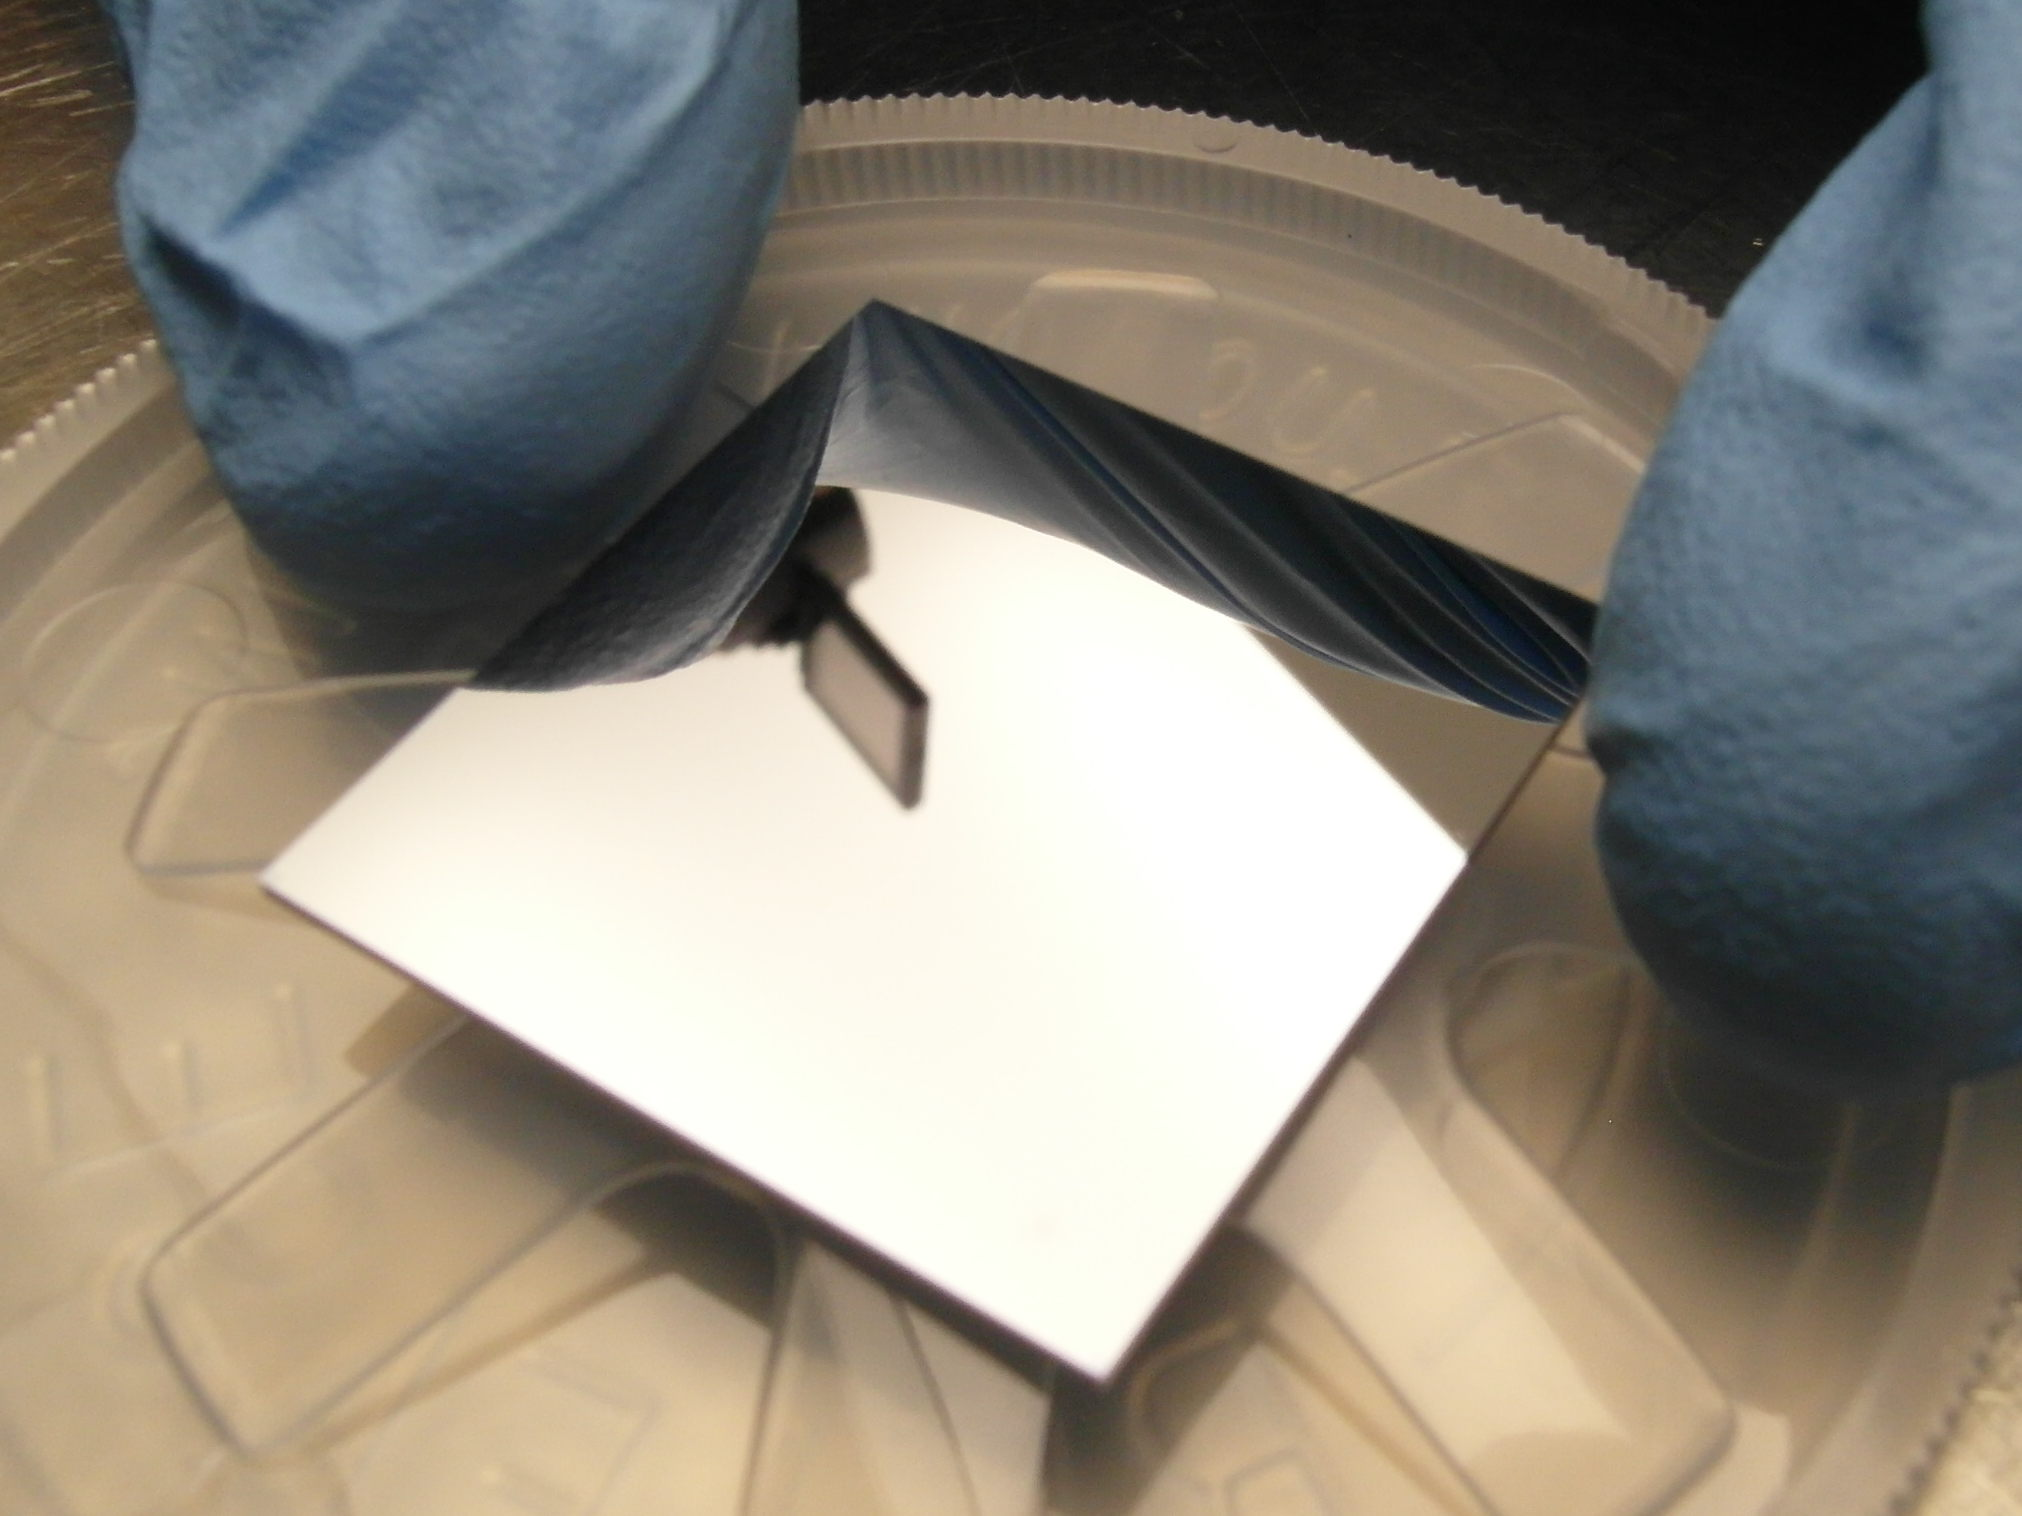
\includegraphics[width=0.4\textwidth]{img/SAM_1910_v1}
        \caption[Mo/Si multilayer sample.]{%
            Photograph of a Mo/Si multilayer mirror sample on $\mm{20} \times \mm{20}$ wafer substrate.}
        \label{ch_exp:fig_mosi_sample}
\end{figure}
In case of the Cr/Sc systems, wafer pieces of varying size but approximately $\mm{10} \times \mm{20}$ served as the substrate.

\section{Analytical Tools}
In this thesis, several experiments are conducted on different sample systems requiring a dedicated analytical toolset to analyze the sets of data and implement the theoretical calculations based on the models introduced in chapter~\ref{ch_theo}. For that purpose, dedicated software was developed to enable the quantitative analysis conduced in the following chapters. Here, an overview of the software packages and their relation to those already existing and integrated into the framework is given.

All software was written in the \emph{Python} programming language using the \emph{Numpy} and \emph{Scipy} frameworks \cite{walt_numpy_2011} for data analysis and scientific computing. The graphical representation of the data and calculations was done using the \emph{Matplotlib} \cite{hunter_matplotlib:_2007} framework.

The packages developed may be coarsely categorized in the calculation of the electromagnetic field inside and outside a multilayer system following the matrix algorithm explained in Sec.~\ref{ch_theo:sec_matrix_algorithm}, the implementation of the \gls{dwba} as described in Sec.~\ref{ch_theo:sec_diffuse_scattering} and the optimization algorithms partly using existing software packages. All modules were combined using the framework provided by \emph{iPython Notebooks} \cite{perez_ipython:_2007}, which allow to integrate the modules necessary to analyze a sample system including the results of the calculations and their graphical representation within a single code file. The individual modules and descriptions of the functions provided by them is listed below.
\begin{description}
 \item[matrixmethod]{Implementation of the matrix algorithm for calculating electromagnetic fields inside a multilayer system. The theoretical fundamentals of this module are described in detail in Sec.~\ref{ch_theo:sec_matrix_algorithm}. The functions provided here require a predefined layer system with the respective optical constants. At each of the interfaces, a roughness/interdiffusion parameter (N\'{e}vot-Croce parameter) may be considered.}
 
 \item[reflectivity]{This module serves as an interface to the \emph{matrixmethod} module. It provides functions to construct a periodic layer system based on the specification of the layer materials, periodicity, densities as well as substrate material. Based on this, the models described in the following chapters can be implemented and the electromagnetic fields outside and inside the systems may be calculated. In addition to the periodic part of the system, capping layers can be considered explicitly. Furthermore, the module provides functions to consider graded interfaces of different thickness by introducing a given amount of sublayers. Those provide an automatic gradual sinusoidal transition from the optical constants of one material to the next in the stack. Based on the resulting model, the reflectiviy depending on angle of incidence and wavelength as well as all field components at each interface are returned. This allows to calculate the reflectivity at any specified photon energy and angle of incidence, but due to the availability of the full field components also the x-ray fluorescence to be expected according to the method described in Sec.~\ref{ch_theo:sec_xrf}.}
 
 \item[helper]{Several often used functions are bundled in this module. This includes the unit conversion from electron volt to wavelength for the impinging radiation, the calculation of the wave vectors and the implementation of Snell's law. In addition, this module contains an interface to the \emph{periodictable}\footnote{The \emph{periodictable} module was developed by the DANSE/Reflectometry team, \url{http://www.reflectometry.org/danse/elements.html}} module to obtain the optical constants for the materials specified for the \emph{reflectivity} module from the Henke database \cite{henke_x-ray_1993}.}
 
 \item[dwba]{Implementation of the \gls{dwba} as introduced in Sec.~\ref{ch_theo:sec_diffuse_scattering}. This module executes the dynamic and semi-kinematic calculations described in the theory part. For that purpose it requires the full set of field amplitudes that are calculated within the \emph{reflectivity} module. In addition, a \gls{psd} function needs to be specified which is calculated within the \emph{integrals} module described below and a vertical correlation length value as well as the off-normal roughness correlation angle $\beta$. The result of those calculations are absolute intensities of diffusely scattered radiation depending on the specified detector distance and solid angle, as well as the incidence and exit angles and wavelengths. The result may thus be directly compared to correspondingly measured data.}
 
 \item[integrals]{Due to the separation of the roughness contributions and the contribution due to the multilayer nature of the sample to the diffusely scattered radiation, a separate calculation of the \gls{psd} is possible as explained in Sec.~\ref{ch_theo:sec_diffuse_scattering} and performed by this module. The input parameters of this calculation are the values for the \gls{rms} roughness, the Hurst factor and a lateral correlation length. The result enters the calculations done in the \emph{dwba} module.}
 
 \item[pso]{Implementation of the \gls{pso} algorithm following the detailed description in the publication by \textcite{carlisle_off--shelf_2001}. The details of the application of this optimization algorithm are described in Sec.~\ref{ch_spec:sec_PTB17}. Due to the implementation of that algorithm within the Python programming language, above modules can be directly incorporated and used during an optimization of theoretical curves based on experimental data. This allows to perform all calculations highly parallelized and achieve reasonable calculation times. The implementation of the parallel computing applied here is provided through the \emph{iPython} toolset.}
 
 \item[fitting]{The most used residual functions for fitting data from \gls{euv} and \gls{xrr} measurements are contained in this model for convenience. This module requires the \emph{reflectivity} module (including the model specifications) and input data with specified angle of incidence and wavelength range.}
\end{description}

Based on the toolset of modules given here, all calculations within this thesis were conducted. As mentioned above, for any given system an \emph{iPython notebook} was created bundling all measured data. The modules above provide the required access to simulate and calculate any reflectivity, fluorescence or diffuse scattering experiment conducted in this work and were optimized for highest possible performance. Within each of the notebooks, residual functions were defined constituting an optimization functional for the individual analysis of a single experiment or any combination of experiments. Here, any parameters defining the respective model are specified and can be varied. All specific systems analyzed within the thesis are described in the respective following chapters in detail. Apart from the \gls{pso} algorithm implemented in the \emph{pso} module, the Python-based implementation \emph{emcee} by \textcite{foreman-mackey_emcee:_2013} of a \gls{mcmc} algorithm was used. Again, for any details of the application of this method I refer the reader to the following chapters. With this purely Python-based architecture, it was possible to accelerate any calculation of reflectivity, diffuse scattering and fluorescence necessary within the optimization algorithms using the paralellization framework provided by \emph{iPython}. For that purpose, several available \emph{Linux} machines distributed across the PTB network were used in parallel to combine their computing power for solving the optimization problems within this work in a reasonable time.
